%5_binomial_distribution.tex
%notes for the course Probability and Statistics COMS10011
%taught at the University of Bristol
%2018_19 Conor Houghton conor.houghton@bristol.ac.uk
%To the extent possible under law, the author has dedicated all copyright
%and related and neighboring rights to these notes to the public domain 
%worldwide. These notes are distributed without any warranty. 

\documentclass[11pt,a4paper]{scrartcl}
\typearea{12}
\usepackage{graphicx}
%\usepackage{pstricks}
\usepackage{listings}
\usepackage{color}


\newif\ifind
\indtrue


\lstset{language=C}
\usepackage{fancyhdr}
\pagestyle{fancy}
\lfoot{\texttt{coms10011.github.com}}
\lhead{COMS10011 5\_binomial\_distribution - Conor}
\begin{document}

\section*{5 Binomial distribution}

Say you roll a dice five times, what is the chance you get exactly
three sixes? There are three parts to working out the
probability. First consider the chance of getting three sixes in the
first three rolls. This is $(1/6)^3$. Next consider the change of
getting not-a-six in the next two rolls. This is $(5/6)^2$. Finally,
we are interested, not in getting three sixes followed by two
not-sixes, we are interested in getting exactly three sixes out of
five rolls, so we also need to count the number of ways of choosing
which three of the five rolls gives a six. Putting all this together
and using $R$ to denote the number of sixes
\begin{equation}
p(R=3)=\left(\begin{array}{c}5\\3\end{array}\right)\left(\frac{1}{6}\right)^3\left(\frac{5}{6}\right)^2=0.032
\end{equation}

This is an example of the \textbf{binomial distribution}; the binomial
distribution is important because it describes the result of multiple
independent trials. In a \textbf{binomial experiment}  
\begin{itemize}
\item There are $n$ identical trials.
\item Each trial has one of two outcomes, which we call success, $S$,
  and failure, $F$.
\item The trials are independent.
\item The random variable of interest, say $R$, is the total number of successes.
\end{itemize}
Lets call the chance of success for an individual trial $p$ and the
probability of failure $q=1-p$. By reasoning similar to that used in
the example above, it is easy to see
\begin{equation}
p_R(r)=\left(\begin{array}{c}n\\r\end{array}\right)p^rq^{n-r}
\end{equation}
Examples are plot in Fig.~\ref{fig_binomial}.

\begin{figure}[htb]
\begin{center}
% GNUPLOT: LaTeX picture with Postscript
\begingroup
  \makeatletter
  \providecommand\color[2][]{%
    \GenericError{(gnuplot) \space\space\space\@spaces}{%
      Package color not loaded in conjunction with
      terminal option `colourtext'%
    }{See the gnuplot documentation for explanation.%
    }{Either use 'blacktext' in gnuplot or load the package
      color.sty in LaTeX.}%
    \renewcommand\color[2][]{}%
  }%
  \providecommand\includegraphics[2][]{%
    \GenericError{(gnuplot) \space\space\space\@spaces}{%
      Package graphicx or graphics not loaded%
    }{See the gnuplot documentation for explanation.%
    }{The gnuplot epslatex terminal needs graphicx.sty or graphics.sty.}%
    \renewcommand\includegraphics[2][]{}%
  }%
  \providecommand\rotatebox[2]{#2}%
  \@ifundefined{ifGPcolor}{%
    \newif\ifGPcolor
    \GPcolorfalse
  }{}%
  \@ifundefined{ifGPblacktext}{%
    \newif\ifGPblacktext
    \GPblacktexttrue
  }{}%
  % define a \g@addto@macro without @ in the name:
  \let\gplgaddtomacro\g@addto@macro
  % define empty templates for all commands taking text:
  \gdef\gplbacktext{}%
  \gdef\gplfronttext{}%
  \makeatother
  \ifGPblacktext
    % no textcolor at all
    \def\colorrgb#1{}%
    \def\colorgray#1{}%
  \else
    % gray or color?
    \ifGPcolor
      \def\colorrgb#1{\color[rgb]{#1}}%
      \def\colorgray#1{\color[gray]{#1}}%
      \expandafter\def\csname LTw\endcsname{\color{white}}%
      \expandafter\def\csname LTb\endcsname{\color{black}}%
      \expandafter\def\csname LTa\endcsname{\color{black}}%
      \expandafter\def\csname LT0\endcsname{\color[rgb]{1,0,0}}%
      \expandafter\def\csname LT1\endcsname{\color[rgb]{0,1,0}}%
      \expandafter\def\csname LT2\endcsname{\color[rgb]{0,0,1}}%
      \expandafter\def\csname LT3\endcsname{\color[rgb]{1,0,1}}%
      \expandafter\def\csname LT4\endcsname{\color[rgb]{0,1,1}}%
      \expandafter\def\csname LT5\endcsname{\color[rgb]{1,1,0}}%
      \expandafter\def\csname LT6\endcsname{\color[rgb]{0,0,0}}%
      \expandafter\def\csname LT7\endcsname{\color[rgb]{1,0.3,0}}%
      \expandafter\def\csname LT8\endcsname{\color[rgb]{0.5,0.5,0.5}}%
    \else
      % gray
      \def\colorrgb#1{\color{black}}%
      \def\colorgray#1{\color[gray]{#1}}%
      \expandafter\def\csname LTw\endcsname{\color{white}}%
      \expandafter\def\csname LTb\endcsname{\color{black}}%
      \expandafter\def\csname LTa\endcsname{\color{black}}%
      \expandafter\def\csname LT0\endcsname{\color{black}}%
      \expandafter\def\csname LT1\endcsname{\color{black}}%
      \expandafter\def\csname LT2\endcsname{\color{black}}%
      \expandafter\def\csname LT3\endcsname{\color{black}}%
      \expandafter\def\csname LT4\endcsname{\color{black}}%
      \expandafter\def\csname LT5\endcsname{\color{black}}%
      \expandafter\def\csname LT6\endcsname{\color{black}}%
      \expandafter\def\csname LT7\endcsname{\color{black}}%
      \expandafter\def\csname LT8\endcsname{\color{black}}%
    \fi
  \fi
  \setlength{\unitlength}{0.0500bp}%
  \begin{picture}(5040.00,3528.00)%
    \gplgaddtomacro\gplbacktext{%
      \csname LTb\endcsname%
      \put(990,440){\makebox(0,0)[r]{\strut{} 0}}%
      \put(990,864){\makebox(0,0)[r]{\strut{} 0.025}}%
      \put(990,1289){\makebox(0,0)[r]{\strut{} 0.05}}%
      \put(990,1714){\makebox(0,0)[r]{\strut{} 0.075}}%
      \put(990,2138){\makebox(0,0)[r]{\strut{} 0.1}}%
      \put(990,2563){\makebox(0,0)[r]{\strut{} 0.125}}%
      \put(990,2987){\makebox(0,0)[r]{\strut{} 0.15}}%
      \put(1122,220){\makebox(0,0){\strut{} 0}}%
      \put(1513,220){\makebox(0,0){\strut{} 2}}%
      \put(1904,220){\makebox(0,0){\strut{} 4}}%
      \put(2296,220){\makebox(0,0){\strut{} 6}}%
      \put(2687,220){\makebox(0,0){\strut{} 8}}%
      \put(3078,220){\makebox(0,0){\strut{} 10}}%
      \put(3469,220){\makebox(0,0){\strut{} 12}}%
      \put(3861,220){\makebox(0,0){\strut{} 14}}%
      \put(4252,220){\makebox(0,0){\strut{} 16}}%
      \put(4643,220){\makebox(0,0){\strut{} 18}}%
    }%
    \gplgaddtomacro\gplfronttext{%
      \csname LTb\endcsname%
      \put(3656,3090){\makebox(0,0)[r]{\strut{}$p$=0.25}}%
      \csname LTb\endcsname%
      \put(3656,2870){\makebox(0,0)[r]{\strut{}gaussian}}%
    }%
    \gplbacktext
    \put(0,0){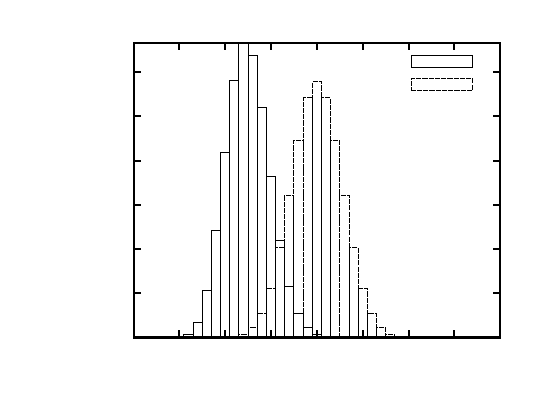
\includegraphics{binomial}}%
    \gplfronttext
  \end{picture}%
\endgroup

\end{center}
\caption{Binomial histograms. Here the value of $p_R(r)$ is plotted where $R$ is a binomial with $n=30$. In the left distribution $p=0.25$ and in the right $p=0.5$.\label{fig_binomial}}
\end{figure}

Say a student is doing a multiple choice vocabulary test in a language
that is very different from the one they speak or any they have never
learned, so they guess all the questions. If there are four options
for each question and fifteen questions, lets calculate $p(5)$, the
chance they get five correct:
\begin{equation}
p(R=5)=\left(\begin{array}{c}15\\5\end{array}\right)(0.25)^5(0.75)^{10}=0.165
\end{equation}

Hopefully you will have seen the binomial coefficient before in the
expansion of polynomials:
\begin{equation}
(q+p)^n=q^n+nq^{n-1}p+\left(\begin{array}{c}n\\2\end{array}\right)q^{n-2}p^2+\ldots+p^n=\sum_{r=0}^n \left(\begin{array}{c}n\\r\end{array}\right)p^rq^{n-r}
\end{equation}
Applied to our case, where $q=1-p$, the left hand side is one; the right hand side is a sum over the probabilities.
\begin{equation}
1=\sum_{r=0}^n \left(\begin{array}{c}n\\r\end{array}\right)p^rq^{n-r}=\sum_{r=0}^np(R=r)
\end{equation}
This is what you would expect, the probabilities should add to
one. However, this formula leads to a very neat trick, first:
\begin{equation}
1=\sum_{r=0}^n \left(\begin{array}{c}n\\r\end{array}\right)p^rq^{n-r}
\end{equation}
Now differentiate both sides with $p$, so take $d/dp$. The left side is a constant so it differentiates to zero and we have
\begin{equation}
0=\sum_{r=0}^n
\left(\begin{array}{c}n\\r\end{array}\right)rp^{r-1}q^{n-r}-\sum_{r=0}^n
  \left(\begin{array}{c}n\\r\end{array}\right)p^r(n-r)q^{n-r-1}
\end{equation}
where we have used the product rule, remembering that $q=1-p$. Next we multiply and divide by either $p$ or $q$, it will be clear why in a few lines time:
\begin{equation}
0=\frac{1}{p}\sum_{r=0}^n \left(\begin{array}{c}n\\r\end{array}\right)rp^rq^{n-r}
-\frac{1}{q}\sum_{r=0}^n \left(\begin{array}{c}n\\r\end{array}\right)p^r(n-r)q^{n-r}
\end{equation}
Now, $n$ is just a constant so we can go
\begin{equation}
\sum_{r=0}^n \left(\begin{array}{c}n\\r\end{array}\right)np^rq^{n-r}=n\sum_{r=0}^n \left(\begin{array}{c}n\\r\end{array}\right)p^rq^{n-r}=n
\end{equation}
Once we deal with this part we see we have two terms that look the same except for the $1/p$ or $1/q$ at the start, 
\begin{equation}
0=\frac{n}{q}-\left(\frac{1}{q}+\frac{1}{p}\right)\sum_{r=0}^n \left(\begin{array}{c}n\\r\end{array}\right)p^rrq^{n-r}
\end{equation}
However, be definition
\begin{equation}
\langle R\rangle=\sum_{r=0}^n p(R=r)r=\sum_{r=0}^n \left(\begin{array}{c}n\\r\end{array}\right)p^rrq^{n-r}
\end{equation}
so
\begin{equation}
\left(\frac{1}{p}+\frac{1}{q}\right)\langle R\rangle=\frac{n}{q}
\end{equation}
It only remains to note
\begin{equation}
\frac{1}{p}+\frac{1}{q}=\frac{q+p}{pq}=\frac{1}{pq}
\end{equation}
to derive
\begin{equation}
\langle R\rangle=pn
\end{equation}

A similar argument based on differentiating twice gives the standard
deviation:
\begin{equation}
\sigma^2=pqn
\end{equation}


\ifind
\section*{Summary}
\else
\subsection*{1 Probability theory}
\fi

\begin{itemize}
\item A \textbf{sample space} is a set of point, they are the possible \textbf{outcomes} of a \textbf{trial}.
\item An \textbf{event} is a subset of a sample space.
\item A \textbf{probability} is a map from events to real numbers such that
  \begin{enumerate}
    \item $P(A)\ge 0$ for all events.
    \item $P(X)=1$
    \item If $A\cap B=\emptyset$ for two events $A$ and $B$ then 
      \begin{equation}
        P(A\cup B)=P(A)+P(B)
      \end{equation}
\end{enumerate}
\item A \textbf{probability mass function} is a map from points in the sample space to real numbers such that
  \begin{enumerate}
\item $p(x)\ge 0$ for all $x\in X$
\item $\sum_{x\in X} p(x)=1$
  \end{enumerate}
\item $P(A)=\sum_{x\in A}p(x)$
\item If all the points in a sample space have the same probability then
  \begin{equation}
P(A)=\frac{\mbox{number of points in }A}{\mbox{number of points in }X}=\frac{\#A}{\#{X}}
  \end{equation}
  where $\#(A)$ means the number of points in $A$.
  \item The \textbf{binomial coefficient}
\begin{equation}
\left(\begin{array}{c}n\\r\end{array}\right)=\frac{n!}{r!(n-r)!}
\end{equation}
counts the number of subsets of size $r$ in a set of $n$ objects and 
\begin{equation}
n!=n\times (n-1)\times (n-2)\times \ldots \times 2 \times 1
\end{equation}
\end{itemize}



\ifind
\section*{Example question}
\else
\subsection*{6 poisson distribution - example question}
\fi
500 meteorites reach the surface of the Earth each year; what is the
chance of five meteorites reaching the surface in a single day.

\noindent \textbf{solution} Well $\lambda=500/365.25$ and so the probability is
\begin{equation}
p(R=5)=\left(\frac{500}{365.25}\right)^5\frac{1}{5!}e^{-500/365.25}\approx 0.01
\end{equation}



\end{document}




